% Данный файл распространяется под лицензией CC BY 4.0. Текст лицензии размещён на https://creativecommons.org/licenses/by/4.0/
% (c) Кафедра системного программирования, 2026
\documentclass[a4paper]{article}

\usepackage[a4paper, top=8mm, bottom=8mm, left=8mm, right=8mm]{geometry}

\usepackage{polyglossia}
\setdefaultlanguage[babelshorthands=true]{russian}
\setotherlanguage{english}

\usepackage{fontspec}
\setmainfont{FreeSerif}
\newfontfamily{\russianfonttt}[Scale=0.7]{DejaVuSansMono}


\usepackage[tiny, compact]{titlesec}

\usepackage{titling}
\setlength{\droptitle}{-1cm}
\pretitle{\begin{center}\begin{bfseries}\Large}
\posttitle{\par\end{bfseries}\end{center}}
\preauthor{\begin{center}\normalsize}
\postauthor{\par\end{center}\vspace{-1.8cm}}

\usepackage{hyperref}
\usepackage{bookmark}
\usepackage{csquotes}
\usepackage{amsmath}
\usepackage{multirow}
\usepackage{graphicx}

\righthyphenmin=2
\lefthyphenmin=2
\hyphenpenalty=50
\pretolerance=5000

\title{Реализация алгоритма PageRank на основе SuiteSparse:GraphBLAS}

\author{Водолазская Елизавета Андреевна}

\date{}

\begin{document}

\maketitle

\begin{flushright}
    Группа: \emph{\enquote{25.Б71-мм}}

    Кафедра: \emph{кафедра Системного программирования}

    Научный руководитель: \emph{Григорьев Семён Вячеславович}

    Консультант: \emph{Кутуев Владимир Александрович}

    Старший инженер-исследователь YADRO

    Номер семестра практики: \emph{2}
\end{flushright}

\section{Введение}
PageRank~--- итерационный алгоритм, предназначенный для оценки относительной важности вершин графа. В основе алгоритма лежит модель случайного блуждания: вероятность нахождения в вершине определяется структурой входящих в неё связей. Формально алгоритм вычисляет стационарное распределение марковской цепи, заданной нормализованной матрицей смежности графа.

PageRank решает задачу количественной оценки центральности узлов в ориентированном графе. Изначально алгоритм был предложен для ранжирования веб-страниц по их значимости на основе гиперссылочной структуры Интернета. В дальнейшем он нашёл применение в задачах анализа социальных сетей, оценки влияния научных публикаций (индексы цитирования), построения рекомендательных систем и других областях, где требуется ранжирование объектов по структуре связей между ними.
\section{Постановка задачи}

\textbf{Целью работы является} реализация алгоритма PageRank на языке C с использованием библиотеки SuiteSparse:GraphBLAS\footnote{URL: \url{https://github.com/DrTimothyAldenDavis/GraphBLAS} (дата обращения: 20.07.2026).} и сравнение производительности собственной реализации с реализацией из библиотеки LAGraph\footnote{URL: \url{https://github.com/GraphBLAS/LAGraph} (дата обращения: 20.07.2026).}.
\textbf{Для достижения цели требуется решить следующие задачи:}
\begin{enumerate}
\item выполнить обзор алгоритма PageRank, стандарта GraphBLAS и существующих реализаций (в частности, библиотеки LAGraph);
\item спроектировать и реализовать итерационный алгоритм PageRank на языке C с использованием алгебраических примитивов для работы с разреженными матрицами;
\item провести проверку корректности реализации и выполнить серию вычислительных экспериментов для сравнения производительности с LAGraph.
\end{enumerate}
\section{Обзор}
GraphBLAS~--- это спецификация, описывающая примитивы линейной алгебры над разреженными матрицами для решения графовых задач. Стандарт определяет набор операций (умножение матрицы на вектор, поэлементные операции, редукции), которые позволяют выражать графовые алгоритмы в терминах матричных вычислений. Основная реализация стандарта на языке C~--- библиотека SuiteSparse:GraphBLAS, разработанная Тимоти Дэвисом.
На базе SuiteSparse:GraphBLAS построена библиотека LAGraph, предоставляющая готовые реализации графовых алгоритмов, включая PageRank, компоненты связности, кратчайшие пути.
Таким образом, для учебной задачи выбрана связка SuiteSparse:GraphBLAS (как базовый инструмент) и LAGraph (как эталон для сравнения). Самостоятельная реализация PageRank позволит изучить применение алгебраических примитивов GraphBLAS к графовым задачам.
\section{Описание предлагаемого решения}

Решение представляет собой библиотеку \texttt{pagerank\_lib} (файлы \texttt{src/pagerank.c}, \texttt{include/pagerank.h}). Функция \texttt{pagerank()} принимает на вход матрицу смежности графа (тип \texttt{GrB\_Matrix}), сохраняет результат в переданном векторе рангов (тип \texttt{GrB\_Vector}) и дополнительно настраивается через параметры алгоритма (коэффициент затухания, точность сходимости, максимальное число итераций). Полное описание интерфейса приведено в документации репозитория\footnote{URL: \url{https://github.com/Lizavod/graphblas-pagerank/blob/main/README.md} (дата обращения: 06.09.2026).}. Используемые технологии: язык C (стандарт C99), SuiteSparse:GraphBLAS версии 7.4.0, CMake версии 3.28.3.

Итерационная формула алгоритма имеет вид:
\begin{equation}
r^{(k+1)} = \alpha \cdot M^T \cdot r^{(k)} + \frac{\alpha \cdot d + (1 - \alpha)}{n} \cdot 1,
\end{equation}
где $M$~--- столбцово-нормализованная матрица смежности, $\alpha$~--- коэффициент затухания, $d$~--- суммарная масса висячих узлов, $n$~--- число вершин, $1$~--- вектор из единиц.

Перед началом итераций выполняется нормализация матрицы смежности: каждый элемент делится на исходящую степень соответствующей вершины. Степени вычисляются с помощью редукции, после чего строится диагональная матрица обратных степеней, и нормализация сводится к одному умножению $M = D_{\text{inv}} \cdot A$.

Особое внимание уделяется висячим узлам (вершинам без исходящих рёбер). Такие узлы имеют нулевую степень, поэтому их масса не перераспределяется через умножение матрицы на вектор и должна быть добавлена отдельно.
Итерационный процесс устроен следующим образом.
\begin{enumerate}
\item \textbf{Вычисление массы висячих узлов.} На каждой итерации из текущего вектора рангов извлекаются значения висячих узлов, после чего их суммарная масса вычисляется с помощью операции редукции.
\item \textbf{Матрично-векторное умножение.} Транспонированная нормализованная матрица смежности умножается на текущий вектор рангов. Транспонирование выполняется без создания копии матрицы.
\item \textbf{Применение затухания и перераспределение.} К результату умножения применяется коэффициент затухания $\alpha$, затем ко всем элементам вектора добавляется константа, учитывающая вероятность телепортации и перераспределённую массу висячих узлов.
\item \textbf{Проверка условий остановки.} Вычисляется L1-норма (сумма модулей элементов вектора, используемая для оценки разности между векторами) разности нового и старого векторов рангов. Итерации завершаются при достижении заданной точности $tol$ или превышении максимального числа итераций $max\_iters$.
\item \textbf{Обновление состояния.} Указатели на векторы текущего и предыдущего состояний меняются местами, что позволяет избежать копирования данных.
\end{enumerate}
\section{Тестирование}
Для проверки корректности реализации разработан набор модульных тестов на 10 синтетических графах малого размера, включающих базовые структуры (цепь, цикл, звезда, полный граф), граничные случаи (одна вершина, две вершины, пустой граф) и проблемные топологии (висячие узлы, несвязный граф, петли).
Проверка выполнялась по двум критериям.
\begin{enumerate}
\item Нормировка вектора рангов:
\begin{equation}
\left| \sum_{i=1}^{n} \text{PR}(v_i) - 1.0 \right| \leq 10^{-6}.
\end{equation}
\item Совпадение с эталонной реализацией LAGraph:
\begin{equation}
\left| \text{PR}_{\text{impl}}(v_i) - \text{PR}_{\text{LAGraph}}(v_i) \right| \leq 10^{-6}, \quad \forall i.
\end{equation}
\end{enumerate}
Тестирование на синтетических графах не выявило ошибок.
\section{Эксперименты}
\subsection{Подготовка к экспериментам}

Для оценки производительности разработанной реализации алгоритма PageRank было проведено сравнение с эталонной реализацией из библиотеки LAGraph. Количество итераций было зафиксировано на уровне, достаточном для получения надёжных и измеримых замеров времени выполнения. В качестве метрики производительности использовалось суммарное время выполнения всех итераций (в секундах). Для каждого графа выполнялось по 30~запусков алгоритма.

Для экспериментов были отобраны пять графов из SuiteSparse Matrix Collection\footnote{URL: \url{https://suitesparse-collection-website.herokuapp.com} (дата обращения: 20.07.2026).}: графы веб-страниц web-Google (916k вершин, 5.1M рёбер) и web-Stanford (282k вершин, 2.3M рёбер), социальный граф hollywood-2009 (1.14M вершин, 113M рёбер), дорожный граф indochina-2004 (7.4M вершин, 194M рёбер) и синтетический граф mycielskian17 (98k вершин, 100M рёбер).

Эксперименты проводились на следующем аппаратном и программном окружении: процессор Intel Core i5-1340P, 16~ГБ оперативной памяти, операционная система Ubuntu 24.04.4 LTS, компилятор GCC 13.3.0. Сборка выполнялась с оптимизацией \texttt{-O3}. Использовались версии библиотек: SuiteSparse:GraphBLAS 7.4.0 и LAGraph 1.2.1.


\subsection{Анализ результатов}

На рисунке~\ref{fig:perf_comparison} представлено сравнение среднего времени выполнения алгоритма. Разработанная реализация показывает большее время выполнения по сравнению с LAGraph на всех тестовых графах. Наибольшее отставание наблюдается на графах \texttt{hollywood-2009} и \texttt{indochina-2004}.

\begin{figure}[h]
    \centering
    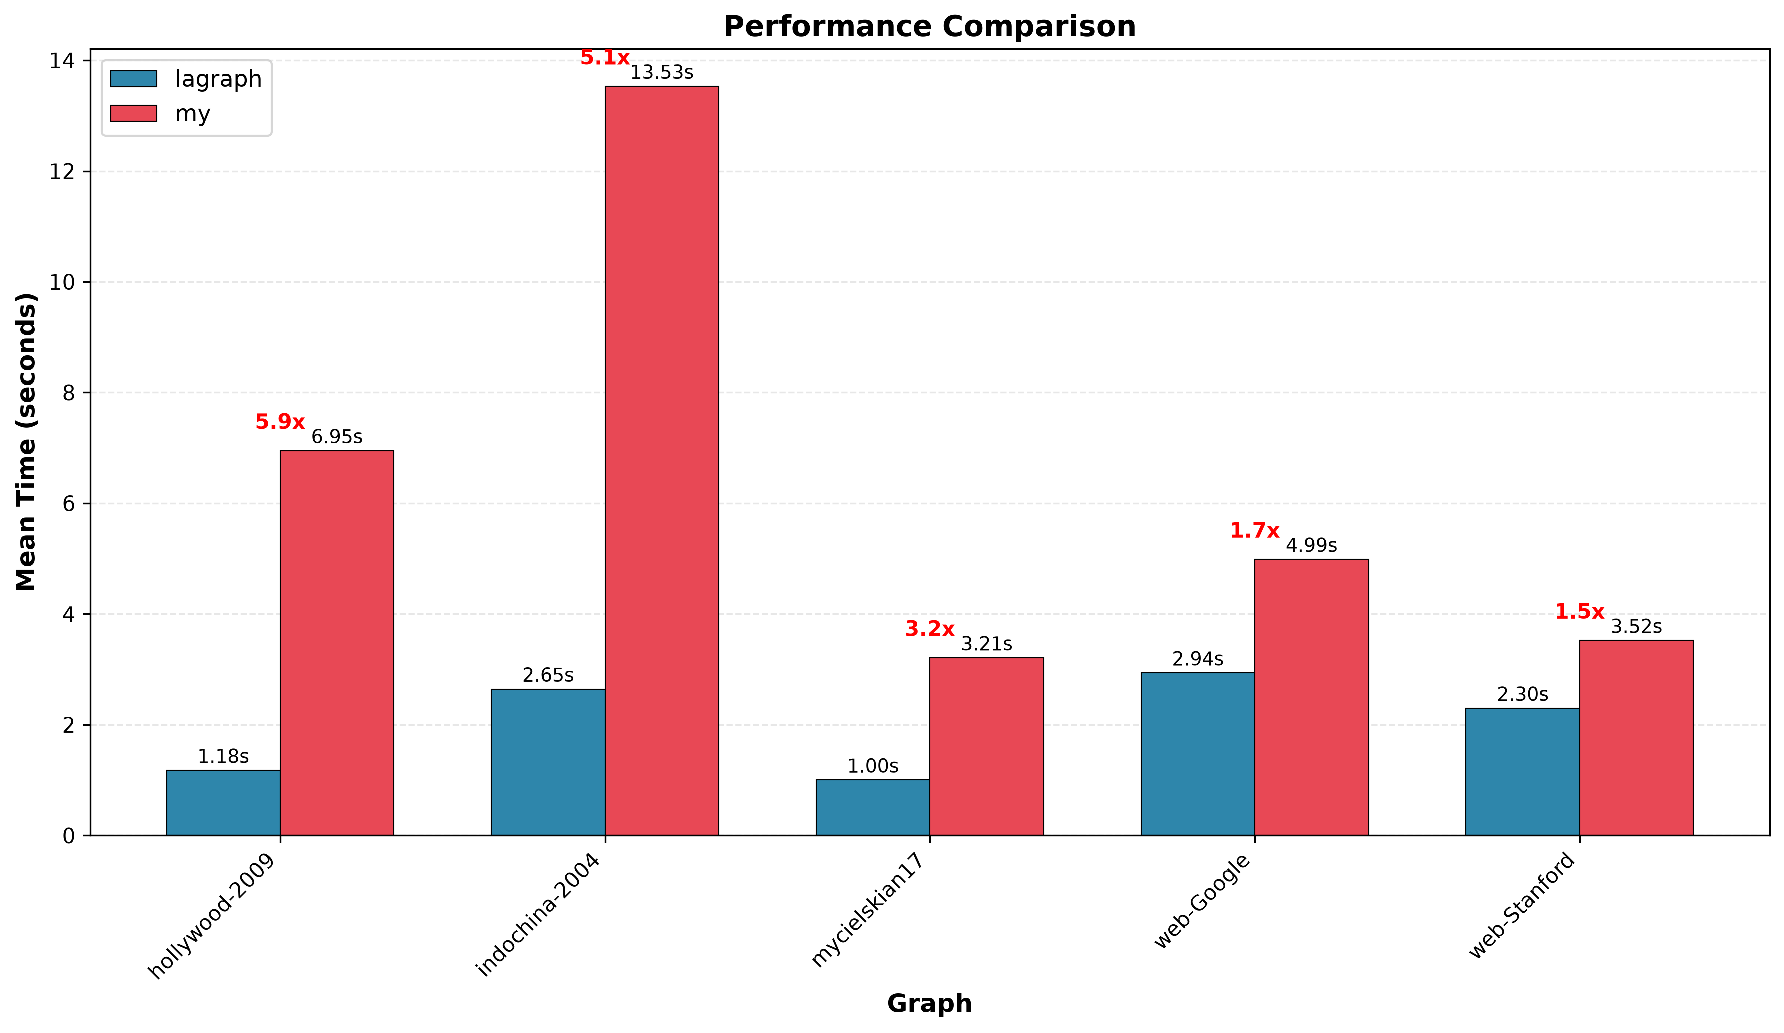
\includegraphics[width=0.75\textwidth]{images/performance_comparison.pdf}
    \caption{Сравнение среднего времени выполнения всех итераций. Числа над столбцами показывают коэффициент замедления.}
    \label{fig:perf_comparison}
\end{figure}


\begin{figure}[h]
    \centering
    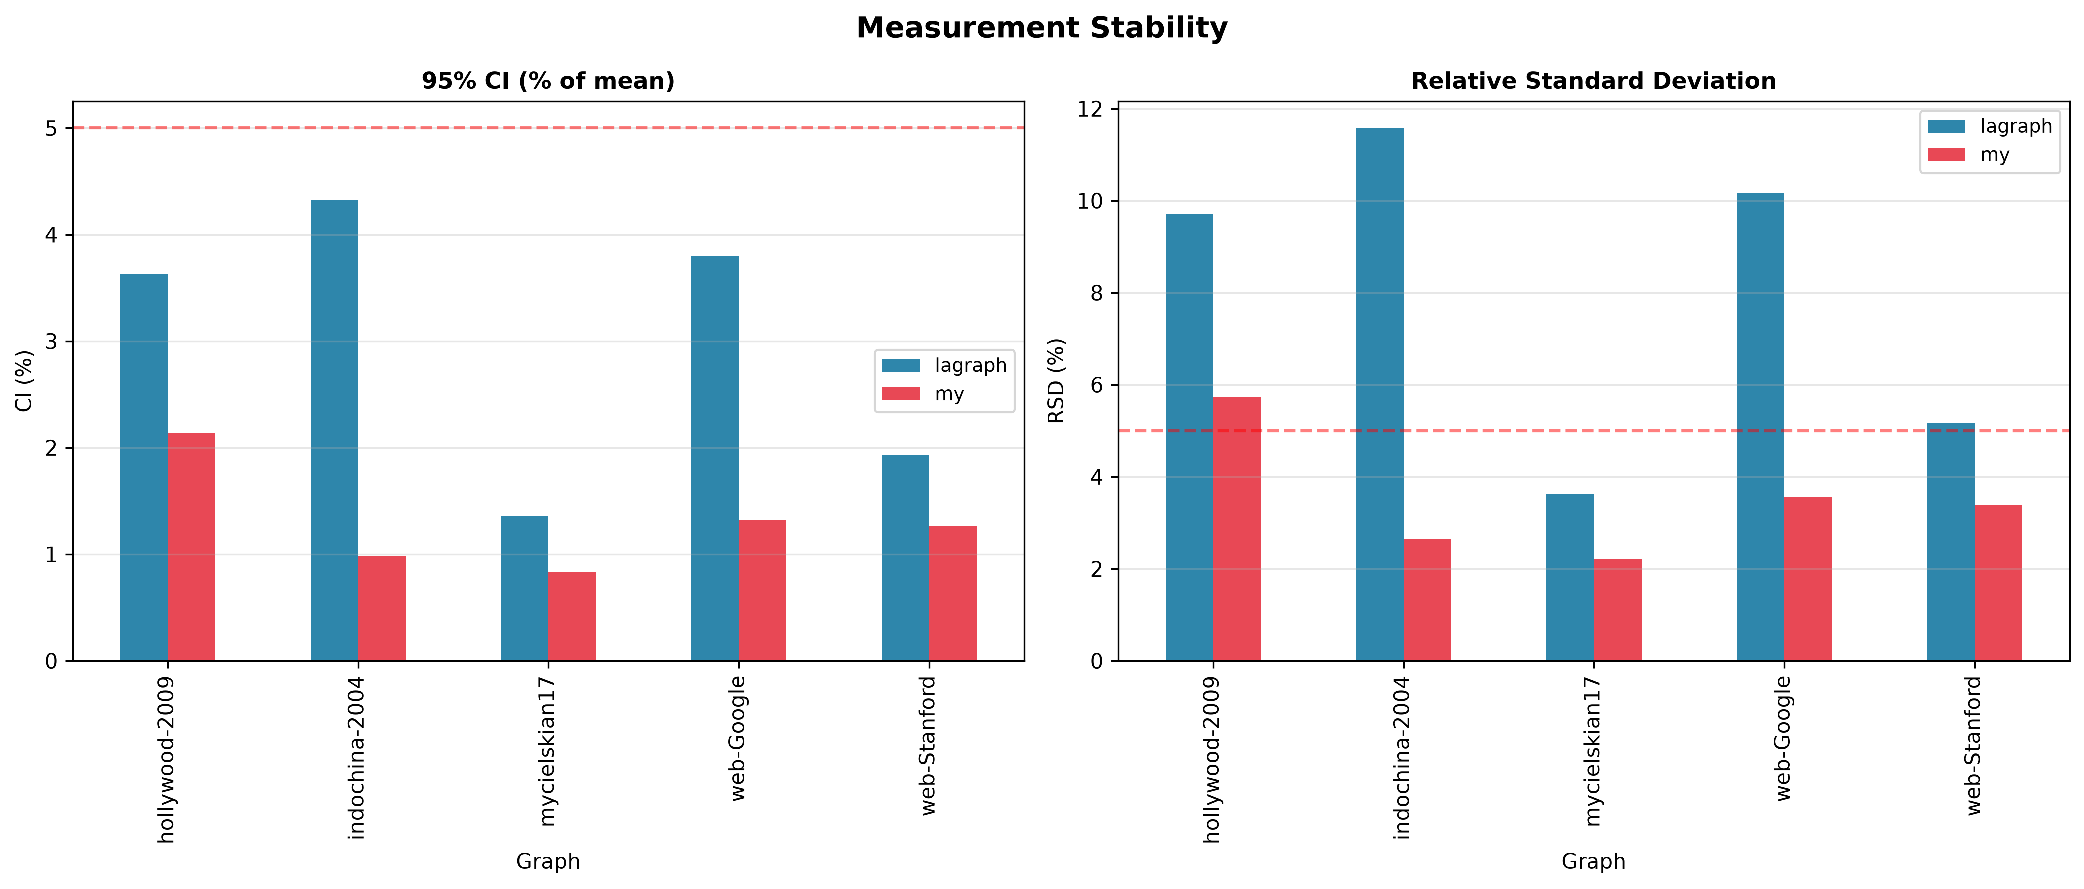
\includegraphics[width=\textwidth]{images/stability.pdf}
    \caption{Анализ стабильности измерений: 95\% доверительный интервал (слева) и относительное стандартное отклонение (RSD) (справа). Пунктирная линия отмечает порог в 5\%.}
    \label{fig:stability}
\end{figure}
Помимо абсолютной скорости, критически важным показателем является стабильность времени выполнения. На рисунке~\ref{fig:stability} проанализированы относительное стандартное отклонение (RSD) и 95\% доверительный интервал (CI) в процентах от среднего значения.

Как видно из графиков, собственная реализация демонстрирует \textbf{более высокую стабильность} по сравнению с LAGraph.
\begin{enumerate}
    \item \textbf{RSD (правый график):} У LAGraph относительное отклонение превышает 5\% для графов \texttt{hollywood-2009} (9.72\%), \texttt{web-Google} (10.17\%) и \texttt{indochina-2004} (11.58\%). У собственной реализации максимальный RSD составляет 5.74\% (\texttt{hollywood-2009}).
    \item \textbf{95\% CI (левый график):} Доверительный интервал собственной реализации стабильно ниже, чем у LAGraph, и не превышает 3\%.
\end{enumerate}

Детальные результаты измерений представлены в репозитории проекта.\footnote{URL: \url{https://github.com/Lizavod/graphblas-pagerank/tree/main/analysis} (дата обращения: 29.07.2026).}

\section{Заключение}
В результате выполнения работы разработана библиотека \texttt{pagerank\_lib}, реализующая алгоритм PageRank с использованием примитивов SuiteSparse:GraphBLAS. Основное внимание уделено применению алгебраического подхода к графовым задачам: нормализация матрицы смежности, работа с висячими узлами и итерационный процесс вычисления рангов выражены через операции над разреженными матрицами и векторами.
Корректность предложенной реализации подтверждена набором тестов на синтетических графах, покрывающих как базовые структуры, так и граничные случаи. Сравнительное тестирование с библиотекой LAGraph показало, что разработанная реализация уступает эталонной по времени выполнения (в 1.5--5.9~раза), однако демонстрирует меньший разброс времени выполнения, что указывает на б\'{о}льшую стабильность измерений.
Полученные результаты позволяют использовать разработанную библиотеку в качестве исследовательского прототипа для изучения применения GraphBLAS к графовым алгоритмам, а также как основу для дальнейшей оптимизации.

Репозиторий проекта: \url{https://github.com/Lizavod/graphblas-pagerank}.

\end{document}